\documentclass[
  bibliography=totoc,     % Literatur im Inhaltsverzeichnis
  captions=tableheading,  % Tabellenüberschriften
  titlepage=firstiscover, % Titelseite ist Deckblatt
]{scrartcl}

% Paket float verbessern
\usepackage{scrhack}

% Warnung, falls nochmal kompiliert werden muss
\usepackage[aux]{rerunfilecheck}

% unverzichtbare Mathe-Befehle
\usepackage{amsmath}
% viele Mathe-Symbole
\usepackage{amssymb}
% Erweiterungen für amsmath
\usepackage{mathtools}

\newcommand{\vek}[2]{\ensuremath{\left( \begin{array}{c}#1\\#2\end{array} \right)}}
\newcommand{\vektor}[3]{\ensuremath{\left( \begin{array}{c}#1\\#2\\#3\end{array} \right)}}
% Fonteinstellungen
\usepackage{fontspec}
% Latin Modern Fonts werden automatisch geladen
% Alternativ:
%\setromanfont{Libertinus Serif}
%\setsansfont{Libertinus Sans}
%\setmonofont{Libertinus Mono}
\recalctypearea % Wenn man andere Schriftarten gesetzt hat,
% sollte man das Seiten-Layout neu berechnen lassen

% deutsche Spracheinstellungen
\usepackage{polyglossia}
\setmainlanguage{german}


\usepackage[
  math-style=ISO,    % ┐
  bold-style=ISO,    % │
  sans-style=italic, % │ ISO-Standard folgen
  nabla=upright,     % │
  partial=upright,   % ┘
  warnings-off={           % ┐
    mathtools-colon,       % │ unnötige Warnungen ausschalten
    mathtools-overbracket, % │
  },                       % ┘
]{unicode-math}

% traditionelle Fonts für Mathematik
\setmathfont{Latin Modern Math}
% Alternativ:
%\setmathfont{Libertinus Math}

\setmathfont{XITS Math}[range={scr, bfscr}]
\setmathfont{XITS Math}[range={cal, bfcal}, StylisticSet=1]

% Zahlen und Einheiten
\usepackage[
  locale=DE,                   % deutsche Einstellungen
  separate-uncertainty=true,   % immer Fehler mit \pm
  per-mode=symbol-or-fraction, % / in inline math, fraction in display math
]{siunitx}

% chemische Formeln
\usepackage[
  version=4,
  math-greek=default, % ┐ mit unicode-math zusammenarbeiten
  text-greek=default, % ┘
]{mhchem}

% richtige Anführungszeichen
\usepackage[autostyle]{csquotes}

% schöne Brüche im Text
\usepackage{xfrac}

% Standardplatzierung für Floats einstellen
\usepackage{float}
\floatplacement{figure}{htbp}
\floatplacement{table}{htbp}

% Floats innerhalb einer Section halten
\usepackage[
  section, % Floats innerhalb der Section halten
  below,   % unterhalb der Section aber auf der selben Seite ist ok
]{placeins}

% Seite drehen für breite Tabellen: landscape Umgebung
\usepackage{pdflscape}

% Captions schöner machen.
\usepackage[
  labelfont=bf,        % Tabelle x: Abbildung y: ist jetzt fett
  font=small,          % Schrift etwas kleiner als Dokument
  width=0.9\textwidth, % maximale Breite einer Caption schmaler
]{caption}
% subfigure, subtable, subref
\usepackage{subcaption}

% Grafiken können eingebunden werden
\usepackage{graphicx}
% größere Variation von Dateinamen möglich
\usepackage{grffile}

% schöne Tabellen
\usepackage{booktabs}

% Verbesserungen am Schriftbild
\usepackage{microtype}

% Literaturverzeichnis
\usepackage[
  backend=biber,
]{biblatex}
% Quellendatenbank
\addbibresource{lit.bib}
\addbibresource{programme.bib}

% Hyperlinks im Dokument
\usepackage[
  unicode,        % Unicode in PDF-Attributen erlauben
  pdfusetitle,    % Titel, Autoren und Datum als PDF-Attribute
  pdfcreator={},  % ┐ PDF-Attribute säubern
  pdfproducer={}, % ┘
]{hyperref}
% erweiterte Bookmarks im PDF
\usepackage{bookmark}

% Trennung von Wörtern mit Strichen
\usepackage[shortcuts]{extdash}

\setlength{\parindent}{0em}

\newcommand{\HRule}{\rule{\linewidth}{0.5mm}}
\newcommand{\pii}{\symup{\pi}}

\author{%
  Janina Nicolini%
  \texorpdfstring{%
    \\%
    \href{mailto:janina.nicolini@tu-dortmund.de}{janina.nicolini@tu-dortmund.de}
  }{}%
  \texorpdfstring{\and}{, }%
  Miriam Schwarze%
  \texorpdfstring{%
    \\%
    \href{mailto:miriam.schwarze@tu-dortmund.de}{miriam.schwarze@tu-dortmund.de}
  }{}%
}
\publishers{TU Dortmund – Fakultät Physik}

\usepackage{wrapfig}

\begin{document}

\begin{titlepage}
  \begin{flushleft}
 Durchführung: 28.05.2019
  \end{flushleft}


\HRule\\[1,0cm]

 \begin{center}

  \textsc{\Large Schwerpunktspraktikum Teilchenphysik \& Detektoren}\\[1,5cm]
\textsc{\LARGE Praktikumsprotokoll}\\[1.5cm]
\textsc{\huge Vermessung von szintillierenden Fasern für das LHCb-Experiment} \\[5,5cm]
%\textsc{Korrektur} \\[5,5cm]

Janina Nicolini\footnotemark[1], \\
Miriam Schwarze\footnotemark[2] \\[1,0cm]



 \end{center}
\HRule

 \vfill

 \footnotetext[1]{\href{mailto:janina.nicolini@tu-dortmund.de}{janina.nicolini@tu-dortmund.de}}
 \footnotetext[2]{\href{mailto:miriam.schwarze@tu-dortmund.de}{miriam.schwarze@tu-dortmund.de}}
\end{titlepage}

\section{Einleitung}

\section{Theorie}

\cite{anleitung}

\section{Durchführung}
Zunächst wird der Datensatz wie in Kapitel \ref{Signal} aufbereitet. Danach lässt sich mit Hilfe der mRMR-Selektion eine Attributsauswahl treffen. Mit den ausgewählten Attributen wird anschließend eine Seperation mit verschiedenen Lernern durchgeführt. Dabei erfolgt die Seperation mit einem Naiven-Bayes-Klassifikator, einen kNN-Klassifikator und einem Random-Forest. \\
Um einen Vergleich der verschiedenen Lerner zu ermöglichen, werden zuletzt die Qualitätsparameter für alle drei Methoden bestimmt und verglichen.

\section{Auswertung}

\subsection{Auswertung der Simulationsdaten}
Da die Simulationsdaten Events enthalten, welche für die Auswertung nicht relevant sind, werden diese zunächst selektiert. Die Verteilung der Selektionsvariablen sind in Abbildung \ref{fig:Cuts_sim} abgebildet.
\begin{figure}
    \centering
    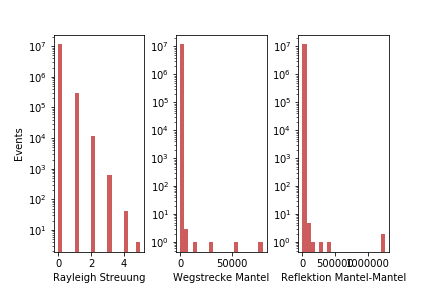
\includegraphics[width=0.5\textwidth]{plots/cuts_sim.pdf}
    \caption{Verteilung der Selektionsvariablen (von links nach rechts): Anzahl Rayleigh-Streuungen, Wegstrecke im Mantelmaterial, Reflektion an der Mantel-Mantel-Grenzfläche.}
    \label{fig:Cuts_sim}
  \end{figure}
  \FloatBarrier
Photonen, welche in der Faser gestreut werden, können nicht mehr durch die in Kapitel \ref{theorie} gefundenen Gleichungen beschrieben werden. Aus diesem Grund werden Ereignisse, deren Anzahl an Rayleigh-Streuungen (\textit{rayleighScatterings}) größer als Null ist, verworfen.
Des Weiteren sollen im Folgenden zwischen Photonen unterschieden werden, welche sich lediglich im Kern bewegen und welche, die in den Mantel reflektiert werden. Die Ersten werden im Folgenden als Kernphotonen bezeichnet, während die Photonen, welche in den Mantel eindringen, Mantelphotonen genannt werden.
Zu den Mantelphotonen zählen die Photonen mit einer Wegstrecke im Mantelmaterial (\textit{length\_clad}) und einer Anzahl an Reflektionen an der Mantel-Mantel-Grenzfläche (\textit{reflClCl}) größer Null. \\

Im Anschluss wird für alle Photonen der Winkel $\theta$ zwischen der $x$-Achse der Faser und ihrer Wegstrecke bestimmt. Anhand von Abbildung \ref{fig:Geometrie} kann der Zusammenhang
\begin{align}
    \vec{p}\vec{e}_{\mathrm{x}} &= |\vec{p}||\vec{e}_{\mathrm{x}}| \cos(\theta) \\
    \Leftrightarrow \theta &= \arccos(p_{\mathrm{x}})
\end{align}
hergeleitet werden. Die Verteilung von $\theta$ für die Kern- und Mantelphotonen ist in Abbildung \ref{fig:theta_sim} dargestellt.
\begin{figure}
    \centering
    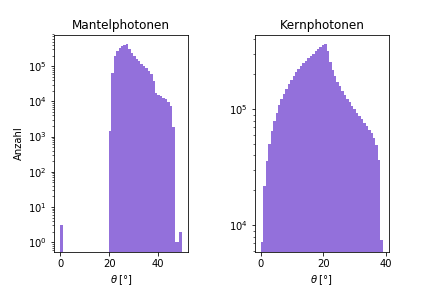
\includegraphics[width=0.5\textwidth]{plots/theta_sim.pdf}
    \caption{Verteilung vom Winkel $\theta$, welcher den Winkel des Photons zur $x$-Achse beschreibt, für die Kern- und Mantelphotonen.}
    \label{fig:theta_sim}
\end{figure}
\FloatBarrier
Die Kernphotonen weisen eine unsymmetrische Verteilung um etwa $\SI{20}{°}$ auf, wobei in dem Bereich oberhalb des Maximums weniger Photonen zu finden sind. Es werden Werte zwischen $\SI{0}{°}$ und $\SI{40}{°}$ angenommen. Die Verteilung der Mantelphotonen hingegen beginnt bei einem Winkel von etwa $\SI{20}{°}$ Grad und nimmt auch Werte etwas oberhalb von $\SI{40}{°}$ an.\\

Mit Hilfe der Histogramme wird das Verhältnis von Kern- und Mantelphotonen für jeden Winkel $\theta$ bestimmt, indem die Anzahl an Einträgen der Mantelphotonen pro Bin durch die Anzahl an Kernphotonen dividiert wird. In Abbildung \ref{fig:ratio_sim} sind die Verhältniswerte in Abhängigkeit von $\theta$ zu erkennen.
\begin{figure}
    \centering
    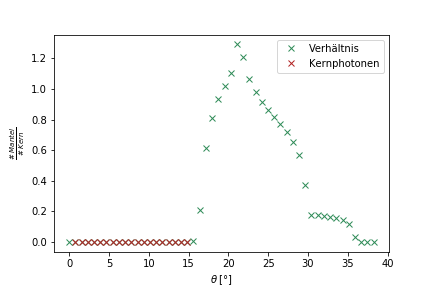
\includegraphics[width=0.5\textwidth]{plots/ratio_sim.pdf}
    \caption{Verhältnis von Kern- und Mantelphotonen in Abhängigkeit vom Winkel $\theta$ (grün). In rot sind die Winkelbereiche gekennzeichnet, in denen nur Kernphotonen auftreten.}
    \label{fig:ratio_sim}
\end{figure}
\FloatBarrier
Ein besonders starkes Vorkommen von Mantelphotonen ist in einem Winkelbereich von etwa $\SI{15}{°}$ bis $\SI{30}{°}$ zu erkennen, wobei sich das Maximum bei einem Winkel von etwa über $\SI{20}{°}$ befindet.

Verhältnisse von Kern- und Mantelphotonen mit dem Wert Null weisen auf Winkelbereiche hin, in denen lediglich Kernphotonen auftreten. Diese Bereiche sind in Abbildung \ref{fig:ratio_sim} mit der Farbe rot gekennzeichnet und treten für Winkelbereiche unterhalb von
\begin{align*}
    \theta_{\mathrm{just core, max}} = \SI{14.82}{°}
\end{align*}
auf. \\

Der minimale Abstand $r_{\mathrm{min}}$ der Kernphotonen zur $x$-Achse kann über den Abstand windschiefer Geraden bestimmt werden. Hierzu wird der Weg des Photons mit der Gleichung
\begin{align}
    p(t) = \left(\begin{array}{c} x\_start \\ y\_start \\ z\_start \end{array}\right)
        + t \left(\begin{array}{c} px\_start \\ py\_start \\ pz\_start \end{array}\right)
\end{align}
und die $x$-Achse mit
\begin{align}
    a(s) = \left(\begin{array}{c} 0 \\ 0 \\ 0 \end{array}\right)
        + s \left(\begin{array}{c} 1 \\ 0 \\ 0 \end{array}\right)
\end{align}
parametrisiert.
Mit Hilfe des orthogonalen Vektors auf die Stützvektoren
\begin{align}
    \vec{n} = \vec{p}\; \times \; \vec{e}_{\mathrm{x}} = \left(\begin{array}{c} 0 \\ pz\_start \\ -py\_start \end{array}\right)
\end{align}
kann die Hilfebende
\begin{align}
    E = pz\_start \cdot y\_start - py\_start \cdot z\_start
\end{align}
konstruiert werden. Der Abstand ist dann schlussendlich durch
\begin{align}
    r_{\mathrm{min}} = \frac{|pz\_start \cdot y\_start - py\_start \cdot z\_start|}{\sqrt{pz\_start ^2 + py\_start^2}}
\end{align}
gegeben. Die Verteilung von $r_{\mathrm{min}}$ ist Abbildung \ref{fig:rmin_sim} zu entnehmen.
\begin{figure}
    \centering
    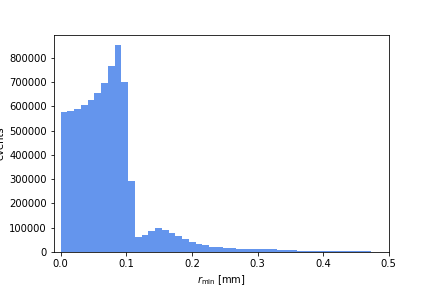
\includegraphics[width=0.5\textwidth]{plots/rmin_sim.pdf}
    \caption{Verteilung des minimalen Abstandes $r_{\mathrm{min}}$ zwischen Photonen und $x$-Achse.}
    \label{fig:rmin_sim}
\end{figure}
\FloatBarrier
Es lässt sich ein gleichmäßiger Anstieg der Verteilung bis zu einem Wert von $r_{\mathrm{min}} \approx \SI{0.1}{mm}$ erkennen, wo die Werte steil abfallen.
Anhand von $r_{\mathrm{min}}$ werden die Kernphotonen auf Daten zugeschnitten, deren $r_{\mathrm{min}}$ kleiner als der Radius der Kernfaser von $\SI{0.1}{mm}$ ist.\\

Zur Bestimmung des mittleren Abstandes pro Winkel werden die $r_{\mathrm{min}}$ in Abhängigkeit von $\theta$ in Abbildung \ref{fig:Hist_rmin_sim} in einem zweidimenesionalen Histogramm aufgetragen.
\begin{figure}
    \centering
    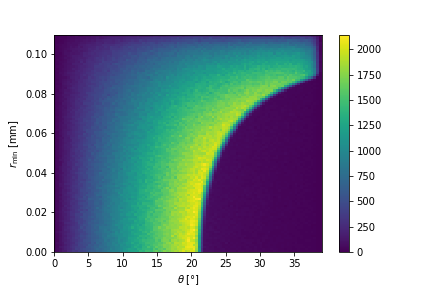
\includegraphics[width=0.5\textwidth]{plots/hist_rmin_sim.pdf}
    \caption{Zweidimenesionales Histogramm der $r_{\mathrm{min}}$ in Abhängigkeit von $\theta$.}
    \label{fig:Hist_rmin_sim}
\end{figure}
\FloatBarrier
Entlang der Achse eines jeden Winkels werden die $r_{\mathrm{min}}$-Werte, gewichtet mit den jeweiligen Einträgen der Histogramm-Matrix, addiert und durch die Summe der Histogramm-Matrixelemente dividiert. Die Mittelwerte von $r_{\mathrm{min}}$ in Abhängigkeit von $\theta$ sind in Abbildung \ref{fig:rmin_mean_sim} zu sehen.
\begin{figure}
    \centering
    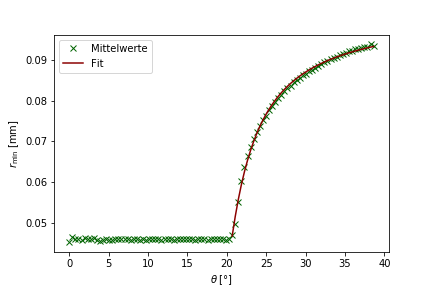
\includegraphics[width=0.5\textwidth]{plots/rmin_mean_sim.pdf}
    \caption{Mittelwerte der $r_{\mathrm{min}}$ in Abhängigkeit vom Winkel $\theta$. }
    \label{fig:rmin_mean_sim}
\end{figure}
\FloatBarrier
Die $r_{\mathrm{min}}$-Werte weisen bis zu einem Winkel von $\theta \approx \SI{20}{°}$ einen konstanten Wert von etwa $\SI{45}{\micro m}$ auf und steigen anschließend an.
In den Anstieg wird eine Fit-Funktion der Form
\begin{align}
    r_{\mathrm{min}}(\theta) = a \arctan(b + c \theta)
\end{align}
gelegt.
Mittels der Funktion \textit{curve\_fit} des Packetes \textit{scipy\_optimize} werden für die Parameter die Werte
\begin{align*}
    a &= (655 \pm 2)\cdot 10^{-4} ,\\
    b &= (-6.5 \pm 0.2),\\
    c &= (358 \pm 9)\cdot 10^{-3}
\end{align*}
ermittelt.

Aus Abbildung \ref{fig:Hist_rmin_sim} wird außerdem der maximale Winkel bestimmt, unter welchem Kernphotonen die Ausleseelektronik erreichen. In Abbildung \ref{fig:theta_max_grad_bsp} ist hierzu der winkelabhängige Verlauf der Photonenintensität beispielhaft für $r_\mathrm{min} = \SI{0.087}{mm}$, sowie der Gradient des Verlaufes dargestellt. Letzterer wird mit der Funktion \textit{numpy.gradient} berechnet. 
\begin{figure}
    \centering
    \includegraphics[width=0.5\textwidth]{plots/theta_max_grad_bsp.pdf}
    \caption{Oben: Verlauf der Photonenintensität in Abhängigkeit des Winkel $\theta$ für $r_\mathrm{min} = \SI{0.087}{mm}$. Unten: Gradient der Photonenintensität in Abhängigkeit des Winkel $\theta$ für $r_\mathrm{min} = \SI{0.087}{mm}$. }
    \label{fig:theta_max_grad_bsp}
\end{figure}
\FloatBarrier
Die Photonenintensität steigt stetig an und fällt anschließend steil auf etwa null ab. An der Stelle des Endpunktes dieses Abfalls ist ein Minimum des Gradienten erkennbar, da die Steigung ab diesem Punkt lediglich flach verläuft. Dieses Verfahren wird für alle $r_\mathrm{min}$-Werte durchgeführt.
Die Grenzwinkel $\theta_{\mathrm{max}}$ sind in Abbildung \ref{fig:theta_max_sim} gegen $r_{\mathrm{min}}$ aufgetragen.
\begin{figure}
    \centering
    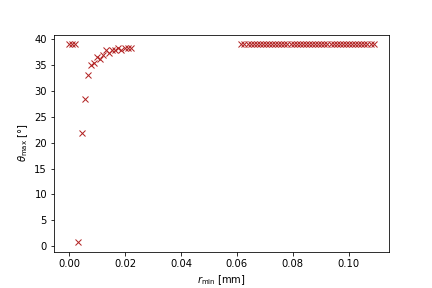
\includegraphics[width=0.5\textwidth]{plots/theta_max_sim.pdf}
    \caption{Grenzwinkel $\theta_{\mathrm{max}}$, unter welchem Photonen noch detektiert werden, in Abhängigkeit vom minimalen Abstand zur Faserlängsachse $r_{\mathrm{min}}$. }
    \label{fig:theta_max_sim}
\end{figure}
\FloatBarrier
Die Werte des maximalen Winkels steigen kontinuierlich zunächst langsam und zu höheren $r_{\mathrm{min}}$-Werten hin steiler an, bevor sie bei $r_\mathrm{min} \approx \SI{0.09}{mm}$ in eine Sättigung von $\theta_{\mathrm{max}}\approx \SI{38}{°}$ übergehen.


Des Weiteren werden die Reflektionswinkel $\theta_{\mathrm{refl}}$ nach Gleichung \eqref{eq:2} berechnet und ihre Verteilung in Abbildung \ref{fig:Theta_refl_sim} in Abhängigkeit vom Winkel $\theta$ aufgetragen.
\begin{figure}
    \centering
    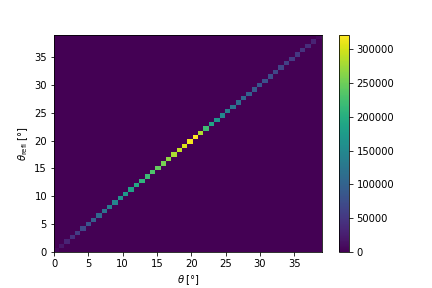
\includegraphics[width=0.5\textwidth]{plots/Theta_refl_sim.pdf}
    \caption{Verteilung der Reflektionswinkel $\theta_{\mathrm{refl}}$ in Abhängigkeit vom Winkel $\theta$. }
    \label{fig:Theta_refl_sim}
\end{figure}
\FloatBarrier
Analog zu den minimalen Abständen $r_{\mathrm{min}}$ werden die Mittelwerte des Reflektionswinkel pro Winkel $\theta$ bestimmt und in Abbildung \ref{fig:Theta_refl_mean_sim} in Abhängigkeit von $\theta$ dargestellt.
\begin{figure}
    \centering
    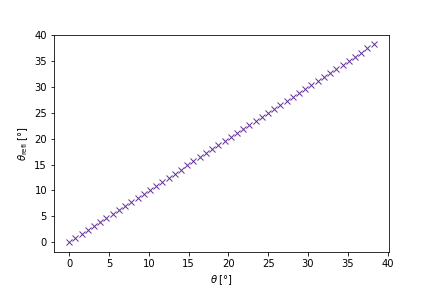
\includegraphics[width=0.5\textwidth]{plots/Theta_refl_mean_sim.pdf}
    \caption{Mittelwerte der Reflektionswinkel $\theta_{\mathrm{refl}}$ in Abhängigkeit vom Winkel $\theta$. }
    \label{fig:Theta_refl_mean_sim}
\end{figure}
\FloatBarrier
Es zeigt sich ein linearer Zusammenhang zwischen dem Reflektionswinkel $\theta_{\mathrm{refl}}$ und dem Winkel des Photons zur Faserachse $\theta$.

Für den Austrittswinkel $\alpha$ der Photonen, welcher über den horizontalen Winkel gemessen wird, kann über Winkelrelationen und das Snellius´sche Brechnungsgesetz der Zusammenhang
\begin{align}
    \alpha = \arcsin \left( \sin(\theta)\frac{n_\mathrm{K}}{n_\mathrm{Si}}\right)
\end{align} 
hergeleitet werden. Hierbei ist der Brechungsindex des Kernes durch $n_\mathrm{K} = 1.6$ \cite{anleitung} und des anschließenden Siliziums durch $n_\mathrm{K} = 3.352$ \cite{si} gegeben.
Die Photonenintensität in Abhängigkeit vom Austrittswinkel ist in Abbildung \ref{fig:austritt_simu} für die Mantel- und Kernphotonen zu erkennen.
\begin{figure}
    \centering
    \includegraphics[width=0.5\textwidth]{plots/austritt_simu.pdf}
    \caption{Anzahl an Photonen als Funktion des Austrittswinkels $\alpha$ für die Mantel- (links) und Kernphotonen (rechts). }
    \label{fig:austritt_simu}
\end{figure}
\FloatBarrier

\subsection{Auswertung der Messdaten}
Zur Überprüfung der Abdunklung des Versuchaufbaus werden die Photonenintensitäten der Untergrundsmessreihen ohne Faseranregung in Abbildung \ref{fig:Untergrund_Untersuchung} in Abhängigkeit von der Wellenlänge $\lambda$ aufgetragen.
\begin{figure}
    \centering
    \includegraphics[width=0.5\textwidth]{plots/Untergrund_Untersuchung.pdf}
    \caption{Photonenintensität durch Hintergrundbeleuchtung in Abhängigkeit von der Wellenlänge $\lambda$ für verschiedene Abdunklungsmaßnahmen.}
    \label{fig:Untergrund_Untersuchung}
\end{figure}
\FloatBarrier
Es lässt sich erkennen, dass für einen Aufbau mit abgedunkelten Raum und abgedecktem Versuchsaufbau der Hintergrund deutlich minimiert werden kann. Dieser Aufbau wird für die weiteren Messungen verwendet. 
Im Vergleich der beiden Winkeleinstellungen lässt sich erkennen, dass die Abschirmung des Hintergrundes nicht für alle Winkel gleich gut funktioniert. 
Für eine weitere Reduzierung des Einflusses der Hintergrundsbeleuchtung wird daher in jeder Messposition der Dunkelstrom aufgenommen und von den gemessenen Photonenintensitäten subtrahiert.

Zur Überprüfung der Radialsymmetrie werden die aufgenommenen Zählraten nach Abziehen des Dunkelstroms für alle Wellenlängen, sowie für jeweils jeden horizontalen und jeden vertikalen Winkel aufsummiert. Die winkelabhängigen Counts sind in Abbildung \ref{fig:radial_test} zu erkennen. 
\begin{figure}
    \centering
    \includegraphics[width=0.5\textwidth]{plots/radial_test.pdf}
    \caption{Aufgenommene Zählrate in Abhängigkeit vom horizontalen Winkel (links) und vertikalen Winkel (rechts) zur Überprüfung der Radialsymmetrie.}
    \label{fig:radial_test}
\end{figure}
\FloatBarrier
Beide Verteilungen lassen eine Radialsymmetrie erahnen, wobei der Mittelpunkt, welcher sich durch einen maximale Photonenintensität auszeichnet, leicht vom Winkel null verschoben ist. Für die folgenden Auswertungsschritte wird von einer radialsymmetrische Verteilung ausgegangen.


Zur Untersuchung der Abschwächung der Photonenintensität entlang der Faser wird zunächst der relevante Wellenlängenbereich ermittelt. Dazu wird die Zählrate in Abhängigkeit von der Wellenlänge beispielhaft für die LED-Position $x = \SI{0}{cm}$ und einen horizontalen Winkel von $\SI{-10}{°}$ aufgetragen. Die gewählten Schnittgrenzen sind in Abbildung \ref{fig:wellenlaengen_cut} durch die gestrichelte Linie gekennzeichnet.
\begin{figure}
    \centering
    \includegraphics[width=0.5\textwidth]{plots/wellenlaengen_cut.pdf}
    \caption{Verteilung der wellenlängenabhängigen Photonenintensität für eine LED-Position von $x = \SI{0}{cm}$ und einem horizontalen Winkel von $\SI{-10}{°}$. In dunkelgrün sind die Schnittgrenzen zur Auswahl des relevanten Wellenlängenbereiches zu erkennen.}
    \label{fig:wellenlaengen_cut}
\end{figure}
\FloatBarrier
Im Folgenden werden Daten aus dem Wellenlängenbereich $\SI{420}{nm} \leq \lambda \leq \SI{640}{nm}$ verwendet.

Die Abschwächung $a_\mathrm{eff}$ ist durch den Zusammenhang 
\begin{align}
    I(x) = I_{0} \exp(a_\mathrm{eff} \cdot x)
    \label{eq:exp_fit}
\end{align}
gegeben, mit der Photonenintensität $I(x)$ bei einer Anregung der Faser an der LED-Position $x$. Zur Berechnung der Abschwächung wird ein mittels der Funktion \textit{curve\_fit} des Packetes \textit{scipy\_optimize} ein Fit der Gleichung \eqref{eq:exp_fit} für jede Wellenlänge und jeden Winkel durchgeführt. Die gefitteten Messpunkte sowie die Fitfunktion sind in Abbildung \ref{fig:Fit_exp_bsp} beispielhaft für eine Wellenlänge von $\lambda = \SI{440.589}{nm}$ und einen horizontalen Winkel von $\SI{-10}{°}$ zu erkennen.
\begin{figure}
    \centering
    \includegraphics[width=0.5\textwidth]{plots/Fit_exp_bsp.pdf}
    \caption{Messpunkte der Photonenintensität in Abhängigkeit von der LED-Position $x$, sowie die Fitfunktion zur Ermittlung der Abschwächung. Beispielhafte Abbildung für eine Wellenlänge von $\lambda = \SI{440.589}{nm}$ und einen horizontalen Winkel von $\SI{-10}{°}$.}
    \label{fig:Fit_exp_bsp}
\end{figure}
\FloatBarrier
Die Fitparameter $I_0$ und $a_\mathrm{eff}$ werden im Anschluss über die Wellenlängen gemittelt und in Abbildung \ref{fig:a_I0_winkel} als Funktion des horizontalen Winkels dargestellt. Der Fehler ergibt sich durch eine Mittelung des Fehlers der Fitparameter.
\begin{figure}
    \begin{subfigure}[c]{0.5\textwidth}    
        \includegraphics[width=0.95\textwidth]{plots/Abschwaechung_winkel.pdf}
        \subcaption{Abschwächung $a_\mathrm{eff}$}    
    \end{subfigure}
    \begin{subfigure}[c]{0.5\textwidth}
        \includegraphics[width=0.95\textwidth]{plots/I0_winkel.pdf}
        \subcaption{Anfangsintensität $I_0$}
    \end{subfigure}
    \caption{Fitparameter $I_0$ und $a_\mathrm{eff}$ in Abhängigkeit des horizontalen Winkels.}
    \label{fig:a_I0_winkel}
\end{figure}

Für die Ermittlung des wellenlängenabhängigen Reflektionskoeffizienten $\epsilon$ wird ein Fit von Gleichung \eqref{eq:9} durchgeführt. Hierzu wird aus dem horizontalen Winkel $\alpha$ der Winkel des Photons zur Faserachse $\theta$ mittels 
\begin{equation}
    \theta = \arcsin \left( \sin(\alpha)\frac{n_\mathrm{Si}}{n_\mathrm{K}}\right)
    \label{eq:theta}
\end{equation}
berechnet. Da die Winkel zur Faserachse $\theta$ relativ sind und keine negativen Werte annimmt, wird der Betrag der Winkelwerte ermittelt. Verwendet werden für den Fit lediglich Kernphotonen, da nur diese durch die im Theorieteil dargestellten Formeln beschrieben werden können. Aus Abbildung \ref{fig:austritt_simu} kann als Grenzwinkel ein horizontaler Winkel von $\alpha \approx \SI{15}{°}$ abgelesen werden.
Für den minimalen Abstand zur Faserachse kann aus Abbildung \ref{fig:rmin_mean_sim} für die verwendeten Winkel ein Mittelwert von $r_\mathrm{min} = \SI{0.06}{mm}$ bestimmt werden, während der Kernradius durch $r_\mathrm{Kern} = \SI{0.11}{mm}$ \cite{anleitung} gegeben ist.
Zur Durchführung des Fits wird nun für jede Wellenlänge die Abschwächung $a_\mathrm{eff}$ in Abhängigkeit vom Winkel $\theta$ aufgetragen und nach Gleichung \eqref{eq:9} gefittet. Dieses ist in Abbildung \ref{fig:fit_a_bsp} beispielhaft für eine Wellenlänge von $\lambda = \SI{440.589}{nm}$ dargestellt.
\begin{figure}
    \centering
    \includegraphics[width=0.5\textwidth]{plots/fit_a_bsp.pdf}
    \caption{Beispielhafte Darstellung des Fits von der Abschwächung $a_\mathrm{eff}$ als Funktion des Winkel $\theta$ zur Ermittlung des Reflektionskoeffizienten $\epsilon$ für $\lambda = \SI{440.589}{nm}$.}
    \label{fig:fit_a_bsp}
\end{figure}
\FloatBarrier
Die Fitparameter $a_0$ und $\epsilon$ sind in Abbildung \ref{fig:a0_epsilon} in Abhängigkeit von der Wellenlänge aufgetragen.
\begin{figure}
    \begin{subfigure}[c]{0.5\textwidth}    
        \includegraphics[width=0.95\textwidth]{plots/a0_lamda.pdf}
        \subcaption{Parameter $a_0$.}    
    \end{subfigure}
    \begin{subfigure}[c]{0.5\textwidth}
        \includegraphics[width=0.95\textwidth]{plots/reflektionskoeff_lamda.pdf}
        \subcaption{Reflektionskoeffizient $\epsilon$.}
    \end{subfigure}
    \caption{Fitparameter $a_0$ und $\epsilon$ als Funktion der Wellenlänge $\lambda$.}
    \label{fig:a_I0_winkel}
\end{figure}

Durch Umstellen von Gleichung \eqref{eq:9} nach $\epsilon$ kann für den Reflektionskoeffizienten als Funktion des Winkels $\theta$ der Zusammenhang 
\begin{align}
    \epsilon = \frac{2\sqrt{r_\mathrm{Kern}^2 -r_\mathrm{min}^2 }}{\tan(\theta)} \left(a_\mathrm{eff}-\frac{a_0}{\cos(\theta)}\right)
    \label{eq:eps}
\end{align}
bestimmt werden. Bei der Berechnung von $\theta$ nach Gleichung \eqref{eq:theta} liefern nicht alle vermessenen Winkel einen zulässigen Wert für $\theta$: Für Austrittswinkel oberhalb von $\SI{20}{°}$ ist Formel \eqref{eq:theta} nicht gültig. 
Für den zulässigen Bereich wird demnach der winkelabhängige Reflektionskoeffizient nach \eqref{eq:eps} berechnet und in Abbildung \ref{fig:reflektionskoeff_winkel} dargestellt. Für einen Winkel von $\theta = \SI{0}{°}$ ergibt sich durch die Division mit Null ein Wert von Unendlich, weshalb dieser ebenfalls vernachlässigt wird. Der Fehler wird mittels der Gauß´schen Fehlerfortpflanzung von $a_\mathrm{eff}$ und $a_\mathrm{0}$ ermittelt.
\begin{figure}
    \centering
    \includegraphics[width=0.5\textwidth]{plots/reflektionskoeff_winkel.pdf}
    \caption{Reflektionskoeffizient $\epsilon$ als Funktion des Winkels zur Faserachse $\theta$. Die Unsicherheiten überdecken einen Teil der Werte.}
    \label{fig:reflektionskoeff_winkel}
\end{figure}
\FloatBarrier
\section{Diskussion}

Die in Abschnitt \ref{kap:Kennlinie} erstellte Kennlinie zeigt in beiden Fällen den erwarteten Verlauf. Die Leckstromwerte der zweiten Messung sind hierbei im Vergleich zur ersten Messung deutlich erhöht. Die zweite Messreihe wurde im Anschluss an die Messungen mit dem Laser aufgenommen. Im Zuge der Bestrahlung mit dem Laser kann sich das Detektormodul erwärmt haben, wodurch die Anzahl der freien Ladungsträger durch thermische Anregung erhöht ist. Hiermit lassen sich die erhöhten Stromwerte erklären.\\

Beide Kennlinien gehen im selben Bereich in einen Sättigungsverlauf über. Die geschätzte Depletionsspannung von $ U_{\mathrm{Dep}} \approx \SI{61}{\volt}$ wird durch die mittels Laser bestimmte Kennlinie in Abschnitt \ref{kap:CCEQ} bestätigt. Die Messungen mittels des Lasers ergeben einen höheren Wert von $ U_{\mathrm{Dep}} \approx \SI{100}{\volt}$. Der Hersteller \textit{Alibavasystems} gibt als Intervall für die Depletionsspannung $\SI{60}{\volt} < U < \SI{80}{\volt}$ an \cite{alibava}. Der im ersten Versuchsteil abgeschätzte Wert liegt innerhalb dieses Intervalles, während der Wert mittels Lasermessung die obere Intervallgrenze deutlich übersteigt.\\

Bei der Untersuchung des Untergrundes in Abschnitt \ref{kap:Pedestal} fällt die Verschiebung der gefundenen Verteilung des Common-Mode-Shifts im Vergleich zur erwarteten Gaußverteilung ins Auge. Ein Fehler in der Aufnahme der ADCC ist an dieser Stelle, wie auch in den weiteren Versuchsteilen auszuschließen, da die Datenaufnahme elektronisch erfolgte.
Vermuten lassen sich an dieser Stelle statistische Schwankungen der Werte. Um diese zu bestätigen oder um die Gaußverteilung der Common-Mode-Shift-Werte um null zu wiederlegen, sollte eine Messung mit einer höheren Eventanzahl durchgeführt werden.\\

Die in Abschnitt \ref{kap:Vermessung} ermittelte \textit{pitch} von $b = \SI{155(25)}{\micro\metre}$ weist eine Abweichung von $\SI{3.125}{\%}$ zur Herstellerangabe von $b_\mathrm{exakt} = \SI{160}{\micro\metre}$ auf \cite{alibava} und stimmt somit relativ gut mit diesem überein. Eine Fehlerquelle kann in der unzureichenden Fokussierung des Lasers gefunden werden. Für die Ausdehnung des Lasers auf dem Sensor wurde ein Wert von $d = \SI{292(17)}{\micro\metre}$ ermittelt, welcher für einen fokussierten Laser relativ hoch erscheint. Aus Abbildung \ref{fig:Position} wird ersichtlich, dass die Laserausdehnung die Breite eines Streifens übersteigt. Dadurch sinkt die Ortsauflösung der Laservermessung und die Positionsbestimmungen werden ungenau.\\

Auch die Berechnung der Eindringtiefe von $a= \SI{179(7)}{\micro\metre}$ über die Länge der an- und absteigenden Flanken wird durch die Ungenauigkeit der Positionsbestimmung beeinflußt.
Aus Abbildung \ref{fig:KennlinieLaser} ist außerdem ersichtlich, dass der Anstieg der CCE relativ zügig erfolgt und daher nur wenige Messwerte durch die Regression beschrieben werden. Für eine exaktere Bestimmung der Eindringtiefe sollten daher mehr Werte unterhalb der Depletionsspannung aufgenommen werden.
Für eine fehlerfreie Vermessung der Sensorstreifen und Lasereigenschaften sollten die Messungen des Weiteren mit einer sorgfältigeren Fokussierung des Lasers wiederholt werden.\\

Einen Einfluss der Laserfokussierung auf die CCE ist nicht zu erwarten, sodass diese Fehlerquelle im Vergleich mit der CCE der $^{90}$Sr-Quelle nicht berücksichtigt werden muss.
Der Energieverlust von Elektronen im Sensor wird durch die modifizierte Bethe-Bloch-Gleichung \ref{eq:12} beschrieben. Die Elektronen der $^{90}$Sr-Quelle gehören mit einer Energie von $\SI{0.546}{\mega\electronvolt}$ zu den minimal ionisierenden Teilchen \cite{periodensystem}. Ihre Energiedeposition im Detektor ist ein statistischer Prozess.
 
Die Intensität der Laserphotonen hingegen sinkt exponentiell mit dem zurückgelegten Weg durch den Streifen. Dieser Zusammenhang führt zu einer Abflachung des Sättigungsverlaufes des Lasers im Vergleich zur Quelle, welches in Abbildung \ref{fig:KennlinieQuelle} zu erkennen ist.

Die in Abschnitt \ref{kap:Quelle} erstellten Energiespektren zeigen den erwarteten Verlauf der Faltung einer Gauß- mit einer Landauverteilung. Laut der Versuchsanleitung \cite{anleitung} beträgt der durchschnittliche Energieverlust von Elektronen in Silizium $\frac{\mathrm{d}E}{\mathrm{d}x} = \SI{3.88}{\mega\electronvolt\per\centi \per \metre}$, was einem durchschnittlichen Energieverlust von $\frac{\mathrm{d}E}{\mathrm{d}x} = \SI{116.4}{\kilo\electronvolt\per 300\; \micro \metre}$ im Streifensensor entspricht. Der bestimmte Mittelwert des Energiespektrums von $\bar{E} = \SI{103.53 \pm 0.06}{\kilo\electronvolt}$ weist eine Abweichung von $\SI{11.06}{\%}$ zu diesem auf. Ein Grund für die Abweichung ist in der Tatsache zu finden, dass es sich bei den Elektronen der $^{90}$Sr-Quelle um minimal ionisierende Elektronen handelt und die durchschnittliche Energiedeposition somit etwas geringer ist. 
%Durch das Verwerfen von Energiedepositionen oberhalb von $\SI{240}{ADCC}$ kann das Spektrum außerdem eine leichte Verschiebung zu kleineren Energiewerten erfahren.


\nocite{*}
\printbibliography

\end{document}
